%!TEX root = ../thesis.tex

\graphicspath{{assets/chapter_2/}}

\chapter{Background}\label{ch:background}

\begin{section}{\glsfmtfull{ris}}
	\begin{subsection}{Programmable Metamaterials}
		Metamaterials refer to artificial structures engineered for unusual properties that may not be found in nature.
		The concept was initially proposed by Victor Veselago in 1967, who conjectured the existence of mediums with negative dielectric constant $\epsilon < 0$ and negative permeability $\mu < 0$ \cite{Veselago1968}.
		Such metamaterials are known as ``negative-index'' because the refraction index is defined as the \emph{negative} square root $n = - \sqrt{\epsilon \mu} < 0$, in order to be consistent with Maxwell's equations.
		It was not until 1999 that their feasibility was experimentally demonstrated by John Pendry at Imperial College using split-ring resonators \cite{Pendry1999}.
		Since then, metamaterials have attracted significant interests due to their counterintuitive properties, to name a few:
		\begin{itemize}
			\item \emph{Negative refraction:} As shown in Fig. \ref{fg:nim_refraction}, the incident and refracted rays stay at the same side of the normal axis \cite{Veselago1968}. This phenomenon is in contrast to the usual refraction but can still be predicted from Snell's law
			\begin{equation}
				\frac{\sin \theta_1}{\sin \theta_2} = n.
			\end{equation}
			It is worth mentioning that a generalized law of refraction and refraction has been proposed in \cite{Yu2011}, which has become a standard reference for the design and analysis of metamaterials.
			\begin{figure}[H]
				\centering
				\subfloat[Negative-index material\label{fg:nim_refraction}]{
					\resizebox{0.45\columnwidth}{!}{
						\input{assets/chapter_2/nim_refraction.tex}
					}
				}
				\subfloat[Positive-index material\label{fg:pim_refraction}]{
					\resizebox{0.45\columnwidth}{!}{
						\tikzstyle{glass}=[color=blue!10]

\tikzset{
	photon/.style={
			draw=black,decorate,
			decoration={snake, segment length=3mm, amplitude=1mm,post length=2mm}
		}
}

% REFLECTION & REFRACTION
\begin{tikzpicture}
	\def\L{7}   % width interface
	\def\l{2}   % length ray
	\def\t{2}   % depth glass gradient
	\def\x{3}   % spacing between plots
	\def\h{1.5}   % bisector height
	\def\f{0.3}   % fraction of interface to the left
	%   \def\na{1.0}  % air
	%   \def\ng{-2}  % glass
	\def\n{0.5}
	\def\anga{45} % angle of incident ray
	%   \def\angg{asin(\na/\ng*sin(\anga))}
	\def\angg{asin(\n*sin(\anga))}
	\coordinate (O) at (0,0);            % point of contact
	\coordinate (I) at (90+\anga:\l);    % point incident (top left)
	\coordinate (M) at (90-\anga:\l);    % point reflected (top right)
	\coordinate (F) at ({-90+\angg}:\l); % point refracted (bottom)
	\coordinate (L) at (-\f*\L,0);       % left point interface
	\coordinate (R) at ({0.5*\L},0);  % right point interface
	\coordinate (T) at (0,\h);           % top middle point (bisector)
	\coordinate (B) at (0,-1.0*\h);      % bottom middle point (bisector)

	\coordinate (T1) at ([shift={(\x,0)}] T);
	\coordinate (B1) at ([shift={(\x,0)}] B);
	\coordinate (I1) at ([shift={(\x,0)}] I);
	\coordinate (O1) at ([shift={(\x,0)}] O);
	\coordinate (F1) at ([shift={(\x,0)}] F);

	% MEDIUM
	\fill[glass] (L) rectangle++ (\L,-\t); % glass gradient
	%   \node[below left=2] at (R) {$n=-2$};
	\node at (1.5,-1.7) {$n=2$};

	% LINES
	\draw[dashed] (T) -- (B); % bisector
	\draw[-latex,black,semithick] (I) -- (O); % incoming ray
	\draw[-latex,black,semithick] (O) -- (F); % refracted ray

	\draw[dashed] (T1) -- (B1); % refracted ray
	\draw[-latex,photon,blue,semithick] (I1) -- (O1); % incoming ray
	\draw[-latex,photon,blue,semithick] (O1) -- (F1); % refracted ray

	% ANGLES
	\draw pic["$\theta_1$",draw=black,angle radius=28,angle eccentricity=1.3] {angle = T--O--I};
	\draw pic["$\theta_2$",draw=black,angle radius=35,angle eccentricity=1.25] {angle = B--O--F};

	% TEXTS
	\node[align=center,below right] at ([shift={(0.3,0)}] O) {Rays\\(energy flow)};
	\node[align=center,below right,blue] at ([shift={(0.3,0)}] O1) {Wave\\vectors};
	%   \draw pic["$\theta_1$",draw=black,angle radius=28,angle eccentricity=1.3] {angle = T1--O1--I1};
	%   \draw pic["$\theta_2$",draw=black,angle radius=35,angle eccentricity=1.25] {angle = F1--O1--B1};

\end{tikzpicture}

					}
				}
				\caption{Refraction in negative and positive-index materials. Incident and refracted rays stay at the same side of the normal axis in a negative-index material.}
			\end{figure}
			\item \emph{Opposite wave direction:} As shown in Fig. \ref{fg:nim_flows}, the wave vector and energy flow (indicated by the Poynting vector) are opposite to each other in a negative-index material \cite{Pendry2004}. This can be inferred from the electric field equation
			\begin{equation}
				\vec{E} = \vec{E}_0 \exp(\jmath k z - \jmath \omega t)
			\end{equation}
			where $k = k_0 n < 0$ is the wavenumber, $\vec{E}_0$ and $k_0$ are the free-space electric field and wavenumber reference, $z$ is the propagation distance, $\omega$ is the angular frequency, and $t$ is the time.
			Negative-index materials are thus also called ``left-hand'' because the propagation direction of the electric and magnetic fields can be determined by a left-hand rule.
			\begin{figure}[H]
				\centering
				\subfloat[Negative-index material\label{fg:nim_flows}]{
					\resizebox{!}{2cm}{
							\input{assets/chapter_2/nim_flows.tex}
					}
				}
				\subfloat[Positive-index material\label{fg:pim_flows}]{
					\resizebox{!}{2cm}{
						\begin{tikzpicture}[background rectangle/.style={fill=blue!10}, show background rectangle]

	\def\f{1/exp(((\x)^2)/2)}

	\begin{axis}[thick,ticks=none,domain=-pi:pi,samples=100,axis x line*=middle,axis y line=none,xlabel=\empty,xmin=-4,xmax=4,ymax=4,ymin=-2]

		\addplot[smooth, color=blue] (\x,{sin((9*(deg(x))) )*\f}) coordinate[pos=0.42] (W);
		\addplot[smooth, color=black] (\x,\f) coordinate[pos=0.6] (E);
		\addplot[smooth, color=black] (\x,-\f);

	\end{axis}
	\draw[-latex,thick] (E) to ++(1,0) node[anchor=west] {energy flow};
	\draw[-latex,thick,blue] (W) to ++(1,0) node[anchor=west,blue] {wave direction};
\end{tikzpicture}

					}
				}
				\caption{Wave and energy have opposite directions in a negative-index material.}
			\end{figure}
		\end{itemize}

		Conventional metamaterials have fixed properties that depend on the geometry and arrangement of their constituent elements.
		Once fabricated, these properties cannot be easily changed unless the structure is physically altered.
		This limits their early usage to military and defense, with applications such as invisibility cloaks and optical illusions.
		In 2014, the concept of ``coding'' and ``programmable'' metamaterials was validated by researchers at Southeast University \cite{Cui2014}, who realized digital control of radar cross-section using biased diodes and \gls{fpga}.
		With a proper model of the target properties and external citation, the metamaterial can be reconfigured in real-time for desired behaviors.
		For example, a self-adaptive metasurface equipped with motion and light sensors have been developed in \cite{Ma2019} for single- and multi-beam steering.

		Next, we discuss the principles of electromagnetic wave redirection via refraction and reflection:
		\begin{itemize}
			\item \emph{Refraction:} As shown in Fig. \ref{fg:nim_focus}, the negative-index material can re-focus the beams diverging from a point source to another point behind the material \cite{Padilla2006}. This could be helpful for wireless applications where the transmitter and receiver are at different sides of the material.
			\item \emph{Reflection:} As shown in Fig. \ref{fg:wave_reflected}, the scattering elements cooperatively alter the phase of the incident wave for a constructive (or destructive) superposition of the reflected waves in the target direction \cite{Poulakis2022}. This could be helpful for wireless applications where the transmitter and receiver are at the same side of the material.
		\end{itemize}
		% electromagnetic wave refraction and reflection.

		\begin{figure}[H]
			\centering
			\subfloat[Negative-index material\label{fg:nim_focus}]{
				\resizebox{0.45\columnwidth}{!}{
						\input{assets/chapter_2/nim_focus.tex}
				}
			}
			\subfloat[Positive-index material\label{fg:pim_diverge}]{
				\resizebox{0.45\columnwidth}{!}{
					\tikzstyle{glass}=[color=blue!10]
\tikzset{
	light beam/.style={decoration={markings,
					mark=at position 0.5 with {\arrow[xshift=3pt]{latex}}},
			postaction={decorate}},
	light beam/.default=0.5}


% REFLECTION & REFRACTION
\begin{tikzpicture}
	\def\w{3.2}     % width interface
	\def\d{1}     % distance between source and glass
	\def\l{3.5}     % distance from glass
	\def\t{2}     % thickness glass
	% \def\na{1.0}  % air
	% \def\ng{2}    % glass
	\def\n{0.5}

\begin{scope}[rotate=90]
	% MEDIUM
	\coordinate (L) at (-\w,-\d);              % lower-left point interface
	\fill[glass] (L) rectangle++ (2*\w,-\t);   % glass

% 	\foreach \anga in {-30,-20,...,30} {
	\foreach \anga in {-30,0,...,30} {
		\pgfmathsetmacro{\angg}{asin(\n*sin(\anga))}

		\pgfmathsetmacro{\a}{\d/cos(\anga)}
		\pgfmathsetmacro{\b}{\t/cos(\angg)}
		\pgfmathsetmacro{\c}{\l/cos(\anga)}

		\coordinate (S) at (0,0);                         % ray source
		\coordinate (I) at (\anga-90:\a);                 % impinging point
		\coordinate (O) at ($(I) + ({\angg-90}:\b)$);     % departing point
		\coordinate (E) at ($(O) + ({\anga-90}:\c)$);     % refraction tail

		% LINES
		\draw[light beam,thick] (S) -- (I);    % incoming ray
		\draw[light beam,thick] (I) -- (O);     % refracted ray in glass
		\draw[light beam,thick] (O) -- (E);     % refracted ray in air
	}
	\node at (-2.6,-2) {$n=2$};
\end{scope}
\end{tikzpicture}

				}
			}
			\caption{Refraction through metamaterials. For negative-index material, beams diverging from a point source is set in reverse and converges back to another point.}
		\end{figure}
		\begin{figure}[H]
			\centering
			\subfloat[Incident wave\label{fg:wave_incident}]{
				\resizebox{!}{4.04cm}{
					\input{assets/chapter_2/wave_incident.tex}
				}
			}
			\subfloat[Reflected wave\label{fg:wave_reflected}]{
				\resizebox{!}{4cm}{
					\begin{tikzpicture}[pics/v/.style={code={\draw (0,-#1) -- (0,#1);}}]
	\begin{scope}
		\clip[overlay] (-5,-5) rectangle (5,0);
		\path[rotate=140,overlay=false,very thick]
		foreach \x in {0,...,9}
			{(-2,-2+0.6*\x) coordinate (L\x) edge[blue,opacity=0,name path global=p\x] ++ (4,0) coordinate (R\x)};
	\end{scope}
	\begin{scope}[xshift=-0.97cm]
		\clip[overlay] (-5,0) rectangle (2.22,-5);
		\pgfmathsetmacro{\myx}{2*cos(30)/cos(30)}
		\path[rotate=203,overlay=false,very thick]
		foreach \x in {0,...,5}
			{(-\myx,0.8+0.6*\x) coordinate (L-\x) edge[green!70!black] ++ (2*\myx,0) coordinate (R-\x)}
		%    (-\myx,-2) edge[gray!30] ++(0,6)
		(\myx,-2) edge[gray!30] ++(0,6)
		%    (0,-2) edge[gray!30] ++(0,7)
		(0,4.5) edge[green!70!black,thick,dashed,latex-] ++ (0,-4);
	\end{scope}
	\path[name path=h] (-5,0) coordinate (L) -- (5,0) coordinate (R);
	\foreach \x in {2,3,4,5}
		{\path[name intersections={of=h and p\x,by=i\x}] (i\x);
			\foreach \y in {1,...,\the\numexpr\x-1}
				{
					\pgfmathtruncatemacro{\myf}{50*(\x-\y)}
					\draw[thick,gray!\myf] (i\x) ++ (-0.18+\y*0.41,0)
					arc[start angle=0,end angle=-180,radius=-0.18+0.41*\y];}}
	\draw (L) -- (R);
	\path foreach \x in {2,3,4,5} {(i\x) node[circle,fill,yellow,inner sep=2pt]{}};

	\begin{scope}[xscale=-1,xshift=-2.5cm]
		\begin{scope}
			\clip[overlay] (-5,-5) rectangle (5,0);
			\path[rotate=140,overlay=false,very thick]
			foreach \x in {0,...,9}
				{(-2,-2+0.6*\x) coordinate (L\x) edge[blue,opacity=0,name path global=p\x] ++ (4,0) coordinate (R\x)};
		\end{scope}
		\begin{scope}[xshift=-0.97cm]
			\clip[overlay] (-5,0) rectangle (2.22,-5);
			\pgfmathsetmacro{\myx}{2*cos(30)/cos(30)}
			\path[rotate=203,overlay=false,very thick]
			foreach \x in {0,...,5}
				{(-\myx,0.8+0.6*\x) coordinate (L-\x) edge[green!70!black] ++ (2*\myx,0) coordinate (R-\x)}
			%    (-\myx,-2) edge[gray!30] ++(0,6)
			(\myx,-2) edge[gray!30] ++(0,6)
			%    (0,-2) edge[gray!30] ++(0,7)
			(0,4.5) edge[green!70!black,thick,dashed,latex-] ++ (0,-4);
		\end{scope}
		\path[name path=h] (-5,0) coordinate (L) -- (5,0) coordinate (R);
		\foreach \x in {2,3,4,5}
			{\path[name intersections={of=h and p\x,by=i\x}] (i\x);
				\foreach \y in {1,...,\the\numexpr\x-1}
					{
						\pgfmathtruncatemacro{\myf}{50*(\x-\y)}
						\draw[thick,gray!\myf] (i\x) ++ (-0.18+\y*0.41,0)
						arc[start angle=0,end angle=-180,radius=-0.18+0.41*\y];}}
		\draw (L) -- (R);
		\path foreach \x in {2,3,4,5} {(i\x) node[circle,fill,yellow,inner sep=2pt]{}};
	\end{scope}

\end{tikzpicture}

				}
			}
			\caption{Reflection through metamaterials. Yellow dots represent scattering elements. Solid and dashed lines denote wavefronts and rays, respectively. The scattering elements work together to manipulate the phases of incident waves, resulting in a focused beam steered in the intended direction.}
		\end{figure}
		It is worth noticing that refraction and reflection are different implementations of \emph{passive beamforming} where the phase and amplitude of the ambient signal are altered by the metamaterial for a desired net effect.
		In the next subsection, we will some typical \gls{ris} scattering models and their physical architecture.
	\end{subsection}

	\begin{subsection}{Wave Scattering Models}
		\begin{subsubsection}{Principles}
			\label{sc:principles}
			\gls{rf} wave can be manipulated by scattering elements made from \emph{programmable metamaterials} or \emph{passive antennas} \cite{Liang2022}.
			As discussed above, the former refracts or reflects the incident signals at the air-cell boundary and mainly applies a phase shift.
			In contrast, the latter allows the wave to feed into and collect from the antenna port such that some energy can be absorbed by the circuit and the rest is reradiated to the space.
			An interesting observation is that when excited by an external wave, a scattering element can simultaneously function as an object and a radiator.
			The corresponding scattered field is \cite{Hansen1989}
			\begin{equation}
				\vec{E}_\text{scatter}(Z_\mathrm{L}) = \underbrace{\vec{E}_\text{structural}}_\text{structural component} + \underbrace{\Gamma I_\mathrm{M} \vec{E}_\text{antenna}}_\text{antenna component},
			\end{equation}
			where $Z_\mathrm{L}$ is the load impedance, $\vec{E}_\text{structural}$ is the residual field under perfect matching (i.e., modelling as an object), $\vec{E}_\text{antenna}$ is the radiated field with unit current at the terminal and no external excitation (i.e., modelling as a radiator), $I_\mathrm{M}$ is the current under perfect matching, and $\Gamma$ is the reflection coefficient
			\begin{equation}
				\Gamma = \frac{Z_\mathrm{L} - Z_0^*}{Z_\mathrm{L} + Z_0},
				\label{eq:reflection_coefficient}
			\end{equation}
			and $Z_0$ is the characteristic impedance for programmable metamaterials or the input impedance for passive antennas.
			It is worth mentioning that
			\begin{itemize}
				\item \emph{Structural component:} Depends on the geometry and material of the scatterer. It is usually modelled as part of the environment multipath \cite{Thomas2012,Liang2020} or simply regarded a \gls{dc} offset when the impinging signal is \gls{cw} \cite{Boyer2014}.
				\item \emph{Antenna component:} Depends on the reflection coefficient that can be altered by load impedance. This is widely exploited for various scattering applications, such as backscatter modulation in \gls{bc} and passive beamforming in \gls{ris} \cite{Zhao2022a}.
			\end{itemize}
			We then introduce two canonical \gls{ris} models that will be adopted in the work chapters.
			More accurate models based on field equations (e.g., \cite{Ozdogan2020,Najafi2020}) and measurement fitting (e.g., \cite{Abeywickrama2020}) are also available in the literature.
			% physics-based (e.g., \cite{Ozdogan2020,Najafi2020}) and practical (e.g., \cite{Abeywickrama2020}) models
		\end{subsubsection}

		\begin{subsubsection}{Diagonal Phase Shift Model}
			A straightforward way to model the \gls{ris} scattering effect is to consider independent scattering elements with purely reactive load impedance \cite{Wu2018}.
			The reflection coefficient of the $n$-th element is thus
			\begin{equation}
				\theta_n = \frac{\jmath X_n - Z^*}{\jmath X_n + Z} = \exp(\jmath \phi_n),
			\end{equation}
			where $X_n$ is the reactance and $\phi_n$ is the phase shift on the scattered wave.
			For a total of $N_\mathrm{S}$ elements, the \gls{ris} scattering matrix is \emph{diagonal with complex unit-magnitude entries}
			\begin{equation}
				\mathbf{\Theta} = \mathrm{diag}(\theta_1, \ldots, \theta_{N_\mathrm{S}}) =
				\begin{bmatrix}
					\theta_1 & 0 & \cdots & 0 \\
					0 & \theta_2 & \cdots & 0 \\
					\vdots & \vdots & \ddots & \vdots \\
					0 & 0 & \cdots & \theta_{N_\mathrm{S}}
				\end{bmatrix}.
			\end{equation}
			Despite the strong assumptions, this diagonal phase shift model is widely used for the analysis of \gls{ris} systems due to its simplicity and analytical tractability.
		\end{subsubsection}

		\begin{subsubsection}{\glsfmtfull{bd} Model}
			How to model the \gls{ris} response if the passive scattering elements can be cooperative instead of independent?
			This question has been answered by \cite{Shen2020a} where a \gls{bd} model was proposed.
			From a network theory perspective \cite{Ivrlac2010}, the interaction between the scattering elements can be modelled as lossless (but not necessarily symmetric) in-group connections in an $N_\mathrm{S}$-port circuit network, as shown in Figs. \ref{fg:bd_ris_architecture_1} and \ref{fg:bd_ris_architecture_2} \cite{Shen2020a}.
			This architecture allows wave impinging on any element to propagate within the circuit and depart partially from other elements in the same group.
			\begin{figure}[H]
				\centering
				\resizebox{0.75\columnwidth}{!}{
					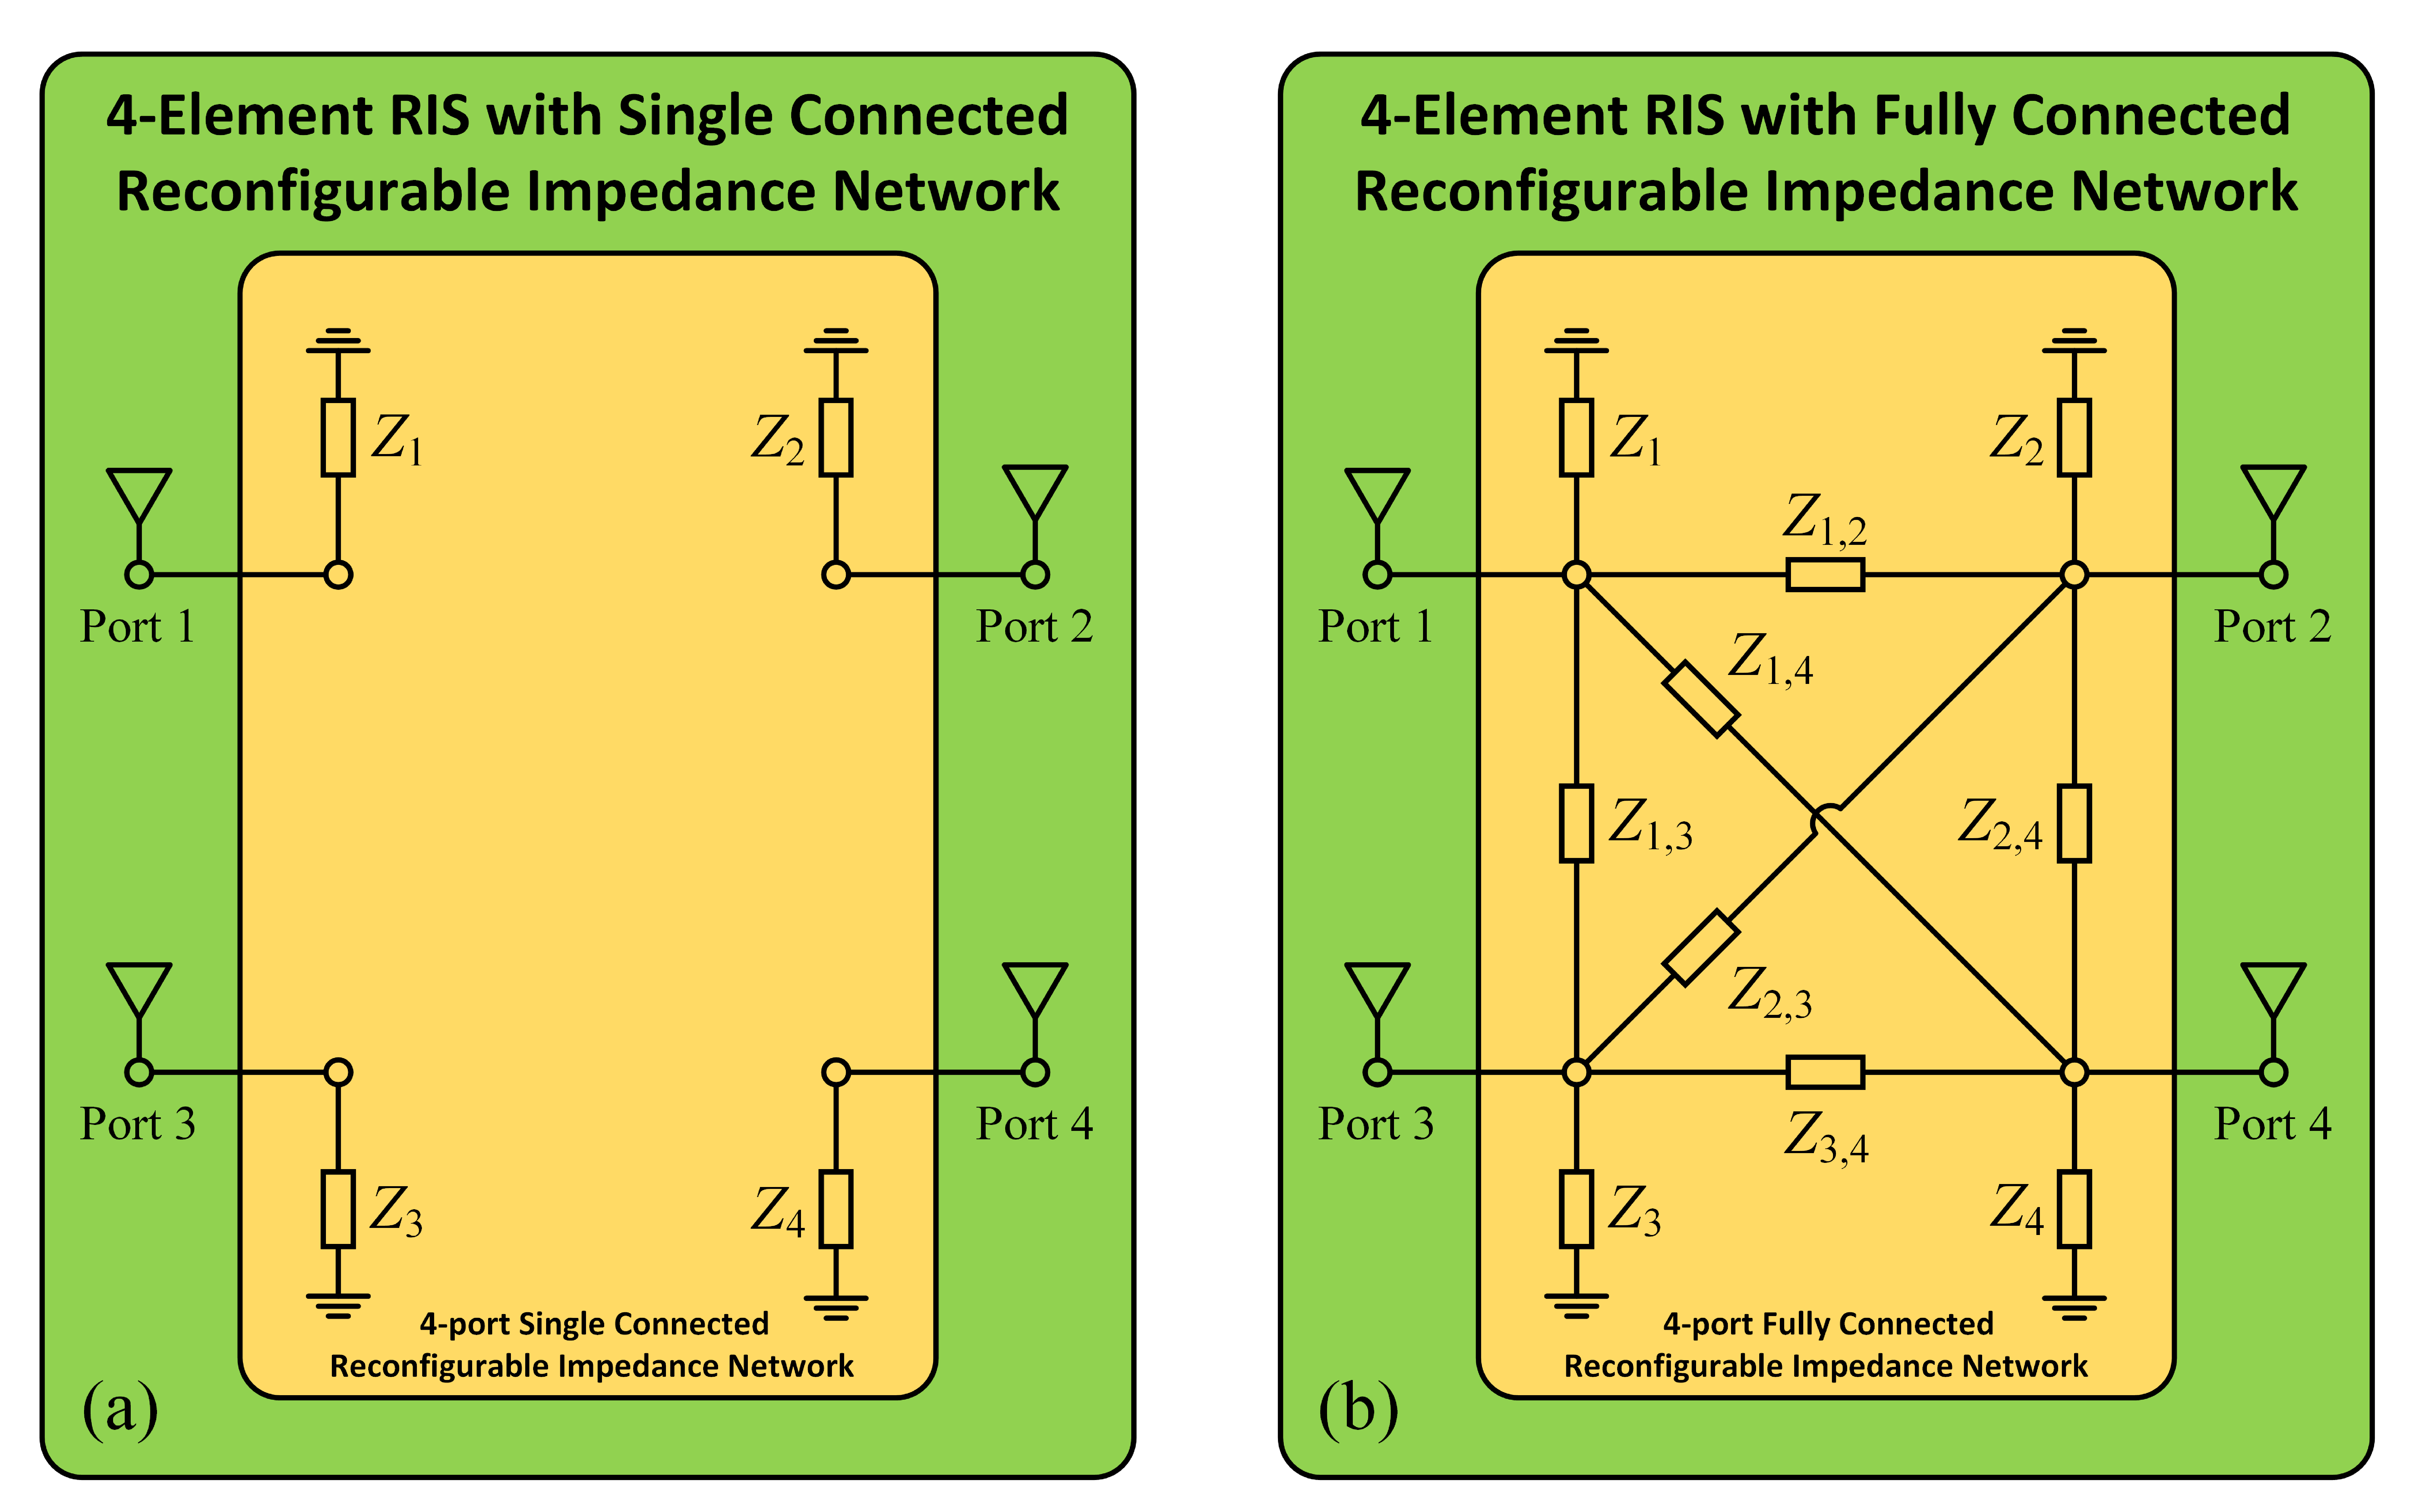
\includegraphics{assets/chapter_2/bd_ris_architecture_1.eps}
				}
				\caption{Network model of a 4-element \gls{ris} with (a) independent scattering and (b) fully cooperative scattering with all elements interconnected. Source: Modified from \cite{Shen2020a}.}
				\label{fg:bd_ris_architecture_1}
			\end{figure}
			\begin{figure}[H]
				\centering
				\resizebox{0.75\columnwidth}{!}{
					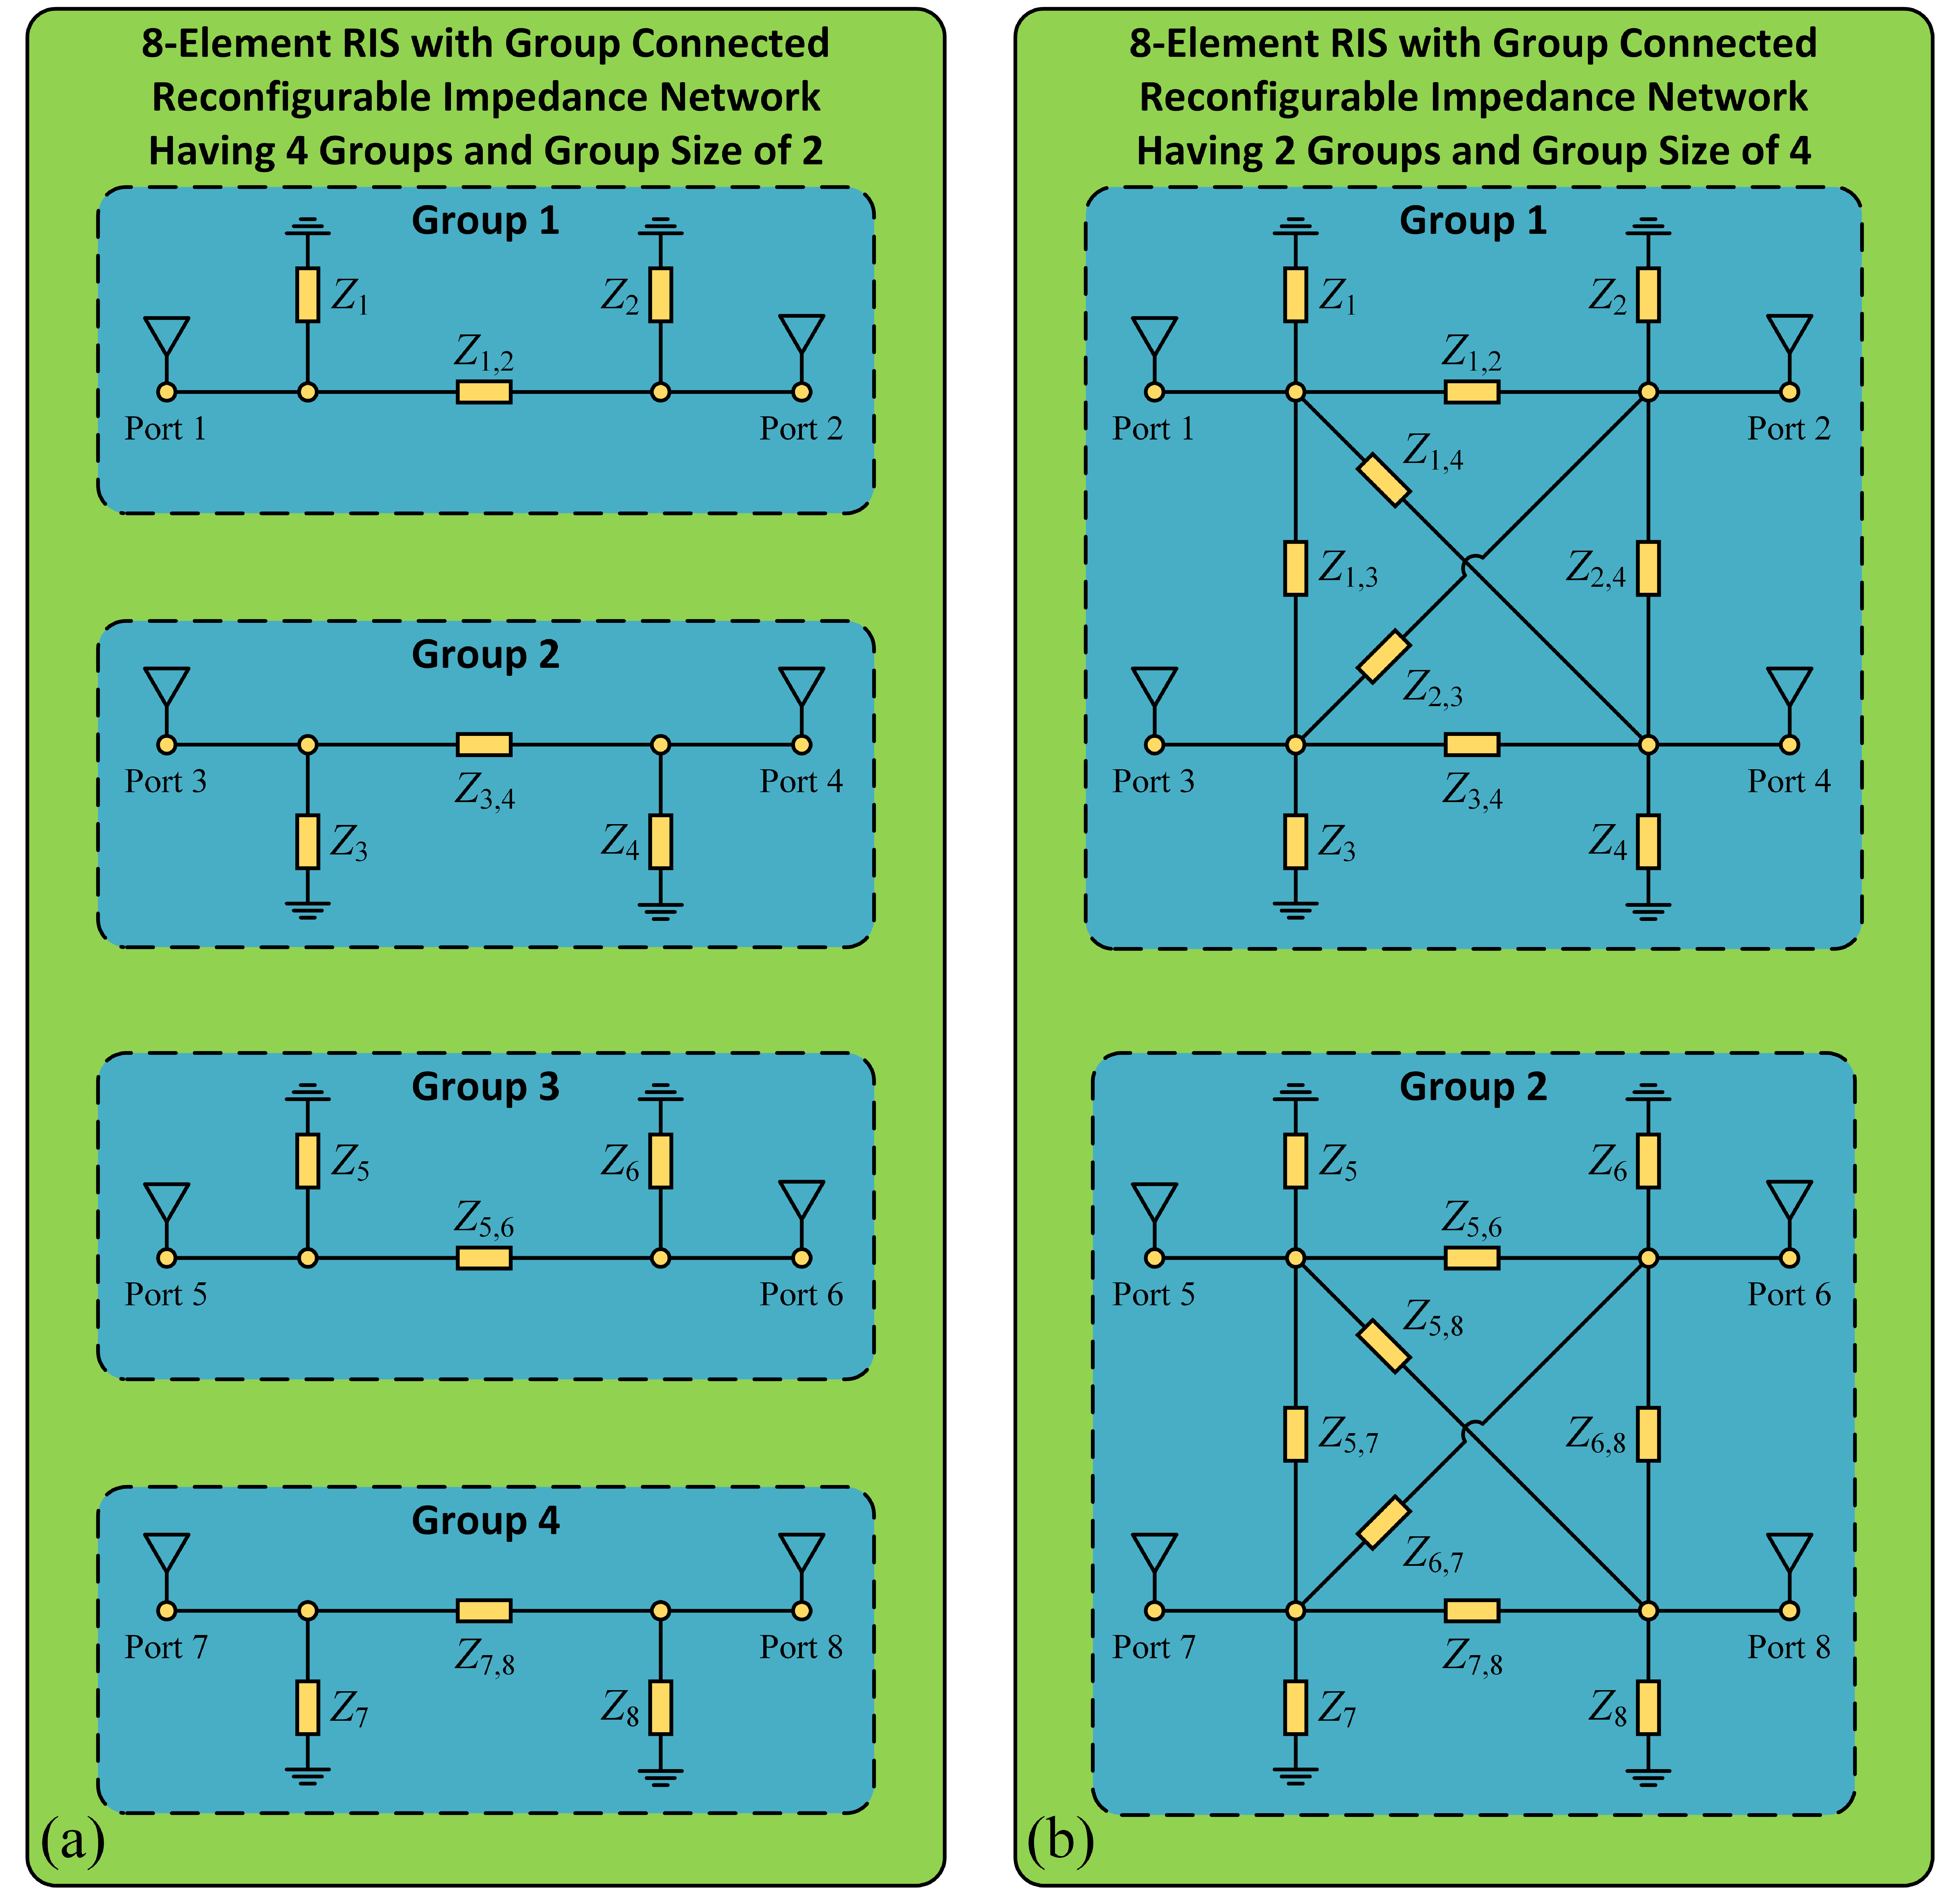
\includegraphics{assets/chapter_2/bd_ris_architecture_2.eps}
				}
				\caption{Network model of an 8-element \gls{ris} with group-wise cooperative scattering of group size (a) 2 and (b) 4. The group size is a design parameter to balance the circuit complexity and scattering performance. Source: Modified from \cite{Shen2020a}.}
				\label{fg:bd_ris_architecture_2}
			\end{figure}

			A general \gls{bd}-\gls{ris} can be modeled as an $N_\mathrm{S}$-port network that divides into $G$ individual groups, each containing $L \triangleq N_\mathrm{S} / G$ elements interconnected by real-time reconfigurable connections.
			With symmetric components (e.g., capacitors and inductors), the scattering matrix of group $g \in \mathcal{G} \triangleq \{1, \ldots, G\}$ is \cite{Shen2020a}
			\begin{equation}
				\mathbf{\Theta}_g = (\jmath \mathbf{X}_g + Z_0 \mathbf{I})^{-1} (\jmath \mathbf{X}_g - Z_0 \mathbf{I}),
			\end{equation}
			which satisfies both \emph{symmetric} and \emph{unitary} properties
			\begin{subequations}
				\begin{equation}
					\mathbf{\Theta}_g = \mathbf{\Theta}_g^\mathsf{T},
					\label{eq:symmetric_property}
				\end{equation}
				\begin{equation}
					\mathbf{\Theta}_g^\mathsf{H} \mathbf{\Theta}_g = \mathbf{I}.
					\label{eq:unitary_property}
				\end{equation}
			\end{subequations}
			On the other hand, lossless networks may also be built over asymmetric passive components (e.g., ring hybrids and branch-line hybrids) \cite{Ahn2006} such that the symmetric constraint \eqref{eq:symmetric_property} can be relaxed.
			This corresponds to the ultimate passive model where energy conservation \eqref{eq:unitary_property} is the only constraint for each group, as widely considered in quantum physics.
			The overall scattering matrix of asymmetric \gls{bd}-\gls{ris} is thus \emph{block-diagonal with unitary blocks}
			\begin{equation}
				\mathbf{\Theta} = \mathrm{diag}(\mathbf{\Theta}_1,\ldots,\mathbf{\Theta}_G) =
				\begin{bmatrix}
					\mathbf{\Theta}_1 & \mathbf{0} & \cdots & \mathbf{0} \\
					\mathbf{0} & \mathbf{\Theta}_2 & \cdots & \mathbf{0} \\
					\vdots & \vdots & \ddots & \vdots \\
					\mathbf{0} & \mathbf{0} & \cdots & \mathbf{\Theta}_G
				\end{bmatrix},
				\label{eq:bd_scattering_matrix}
			\end{equation}
			where \eqref{eq:unitary_property} is equivalently denoted as $\mathbf{\Theta}_g \in \mathbb{U}^{L \times L}$.
			The group size $L$ is a design parameter to balance the circuit complexity and scattering performance.
			Diagonal (single-connected) and unitary (fully-connected) \gls{ris} can be viewed as extreme cases with group size $L=1$ and $L=N_\mathrm{S}$, respectively.
			Therefore, the \gls{bd} model \eqref{eq:bd_scattering_matrix} is envisioned to be the next-generation theoretical foundation for passive \gls{ris}, which grants more design freedom and stronger signal processing capability.

			It is also worth mentioning that each group can be abstracted as a mathematical graph with $L$ vertices and a variable number of edges \cite{Nerini2023a}.
			One element is in the same group with another if and only if there is at least one path (via edges) between them.
			It implies that instead of connecting every pair of elements, the practical circuit can be designed to have a sparse graph with only a few connections, which is beneficial for reducing the circuit complexity and power loss from non-ideal components.
			Antenna directivity and radiation pattern should also be modelled in the scattering matrix, especially when the locations of users or \gls{ris} are not fixed.
			This has motivated the concept of \gls{star}-\gls{ris} \cite{Mu2021,Liu2021} and multi-sector \gls{ris} \cite{Li2023c} where incident wave is partially steered to various directions for different users.
		\end{subsubsection}
	\end{subsection}
\end{section}

\begin{section}{\glsfmtfull{wpt}}
	\begin{subsection}{Introduction}
		Wireless devices are becoming smarter as well as more energy-efficient and eco-friendly.
		Koomey's law \citep{Koomey2011} predicts the computing efficiency roughly doubles every 19 months and the amount of power needed for the same operation decreases to 1\% in a decade.
		Over the past 15 years, the rise of low-power technologies like \gls{wsn} and \gls{iot} have hatched life-changing applications including smart homes, digital healthcare, and industrial automation.
		% This low-power trend has been accelerated by the rise of \gls{iot} and \gls{wsn} technologies, which enabled revolutionary applications including smart homes, digital healthcare, and industrial automation.
		Today, \gls{rfid} tags and basic sensors (e.g., thermometer and proximeter) can operate on microwatts of power \cite{Huang2019,Hao2018}, while communication protocols like \gls{ble} and \gls{lorawan} only consume tens of milliwatts \cite{Correia2017b}.
		This low-power trend together with the upsurge of mobile devices is calling for a \emph{truly wireless} energy solution that eliminates the need for periodic cable plugging or battery replacement.
		% While solutions like solar and piezoelectric offer benefits in specific scenarios, their bulky components, unpredictable power sources, and limited range make them unsuitable for most wireless applications.
		While great successes have been witnessed for candidates like solar and piezoelectric, their prospects in wireless systems remain unclear due to the bulky converter, unpredictable source, and limited operation range.
		One promising solution on the horizon is \gls{wpt} through electromagnetic waves.
		It can be classified into two categories based on the operation principle \cite{Zhou2022}:
		\begin{itemize}
			\item \emph{Non-radiative near-field:} Power is transferred over a short distance (typically a few centimeters) by inductive coupling between coils or capacitive coupling between electrodes in a field-to-field manner. The former has been widely standardized (e.g., Qi 2.0) and commercialized (e.g., wireless charging pads), while the latter is still in the research stage.
			\item \emph{Radiative far-field:} Power is transferred over a long distance (typically a few meters) by directional microwave or laser beams between antennas in a point-to-point manner. It shares many similarities with \gls{rf} communication (e.g., infrastructure and wireless environment) but suffers from lower energy efficiency than non-radiative \gls{wpt} due to pathloss.
		\end{itemize}

		Radiative \gls{wpt}\footnote{In the following part of the thesis, \gls{wpt} refers to radiative \gls{wpt}.} brings numerous opportunities to future wireless networks.
		First, it completely eliminates wired connections and can be integrated into existing wireless systems with minimum modifications.
		Those properties translate to simple deployment, high scalability, and low maintenance cost.
		Second, the power can be simultaneously radiated to multiple devices on demand in a predictable, sustainable and reliable manner.
		This supports our initial vision and is different from other uncontrollable and intermittent energy sources.
		Third and most importantly, radio waves carries power and information simultaneously.
		\gls{wpt} can therefore be jointly designed with \gls{wit} to make the most of radiation, spectrum and infrastructures.
		However, energy efficiency and safety concerns have been two major obstacles that limit the practical development of \gls{wpt}.
		In Section \ref{sc:swipt}, we will discuss how \gls{ris} can help address these issues.
	\end{subsection}

	\begin{subsection}{Modules and Coupling Effect}
		\begin{figure}[H]
			\centering
			\resizebox{\columnwidth}{!}{
				\begin{circuitikz}[transform shape,align=center,font=\footnotesize]
	\draw(0,0) node[draw](rf){\gls{rf}\\source};
	\draw(rf.east) node[txantenna]{};
	\draw(1,1) node{Tx};
	\draw(4.875,2) node[draw]{\gls{ris}};
	\draw(4.875,1) node[draw]{Channel};
	\draw(10,0) node[draw](mc){Matching\\network};
	\draw(mc.west) node[rxantenna,xscale=-1]{};
	\draw(8.7,1) node{Rx};
	\draw(mc.east) to ++(0.85,0) node[anchor=west,draw](d){Diode};
	\draw(d.east) to ++(0.85,0) node[anchor=west,draw](lpf){Low-pass\\filter};
	\draw(lpf.east) to ++(1,0) node[anchor=west,draw](dd){\gls{dc}-\gls{dc}\\converter};
	\draw(dd.east) to ++(1,0) node[anchor=west,draw](s){Storage};

	\draw [dashed] (-0.95,-0.75) rectangle (3.75,2.75);
	\draw (1.4,3) node[]{Energy transmitter};
	\draw [dotted] (6.25,-0.5) rectangle (15.6,2.5);
	\draw (10.925,2) node[]{Rectenna};
	\draw [dotted] (16,-0.5) rectangle (20.5,1.25);
	\draw (18.25,0.875) node[]{Power management unit};
	\draw [dashed] (6,-0.75) rectangle (20.75,2.75);
	\draw (13.375,3) node[]{Energy receiver};

	\draw (-0.95,-1) node[]{$P_{\mathrm{DC}}^{\mathrm{T}}$};
	\draw (3.75,-1) node[]{$P_{\mathrm{RF}}^{\mathrm{T}}$};
	\draw (6,-1) node[]{$P_{\mathrm{RF}}^{\mathrm{R}}$};
	\draw (15.8,-1) node[]{$P_{\mathrm{DC}}^{\mathrm{R}}$};
	\draw (20.5,-1) node[]{$P_{\mathrm{DC}}^{\mathrm{S}}$};

	\draw[gray,dashdotted,-latex] (10.925,-0.5) to ++(0,-1.5) to ++(-1,0) node[anchor=east,draw](c){Channel\\feedback};
	\draw[gray,dashdotted,latex-] (1.4,-0.75) to ++(0,-1.25) to ++(1,0) node[anchor=west,draw](s){Signal\\optimization};
	\draw[gray,dashdotted,-latex] (c.west) to (s.east);
	\draw[gray] (6.45,-2) node[]{Reverse\\communication link};
\end{circuitikz}

			}
			\caption{Block diagram of a closed-loop \gls{ris}-aided \gls{wpt}.}
			\label{fg:wpt_architecture}
		\end{figure}

		The block diagram a closed-loop \gls{ris}-aided \gls{wpt} system is illustrated in Fig. \ref{fg:wpt_architecture}.
		The \gls{rf} signal is generated and radiated by the energy transmitter, propagated through a wireless channel in the presence of a \gls{ris}, captured by the antenna(s) at the receiver, converted to \gls{dc} power by rectifier(s), then passed to the power management unit.
		Upon successful harvesting, the \gls{dc} power is either delivered directly to the device or stored in a battery/super capacitor for future operations.
		When a feedback link is available, one can acquire \gls{csi} at the energy transmitter and exploit it for signal optimization.
		Such a closed-loop \gls{ris}-aided \gls{wpt} system can provide a complete control of transmitter, channel, and receiver, which is essential for maximizing the end-to-end power transfer efficiency
		\begin{equation}
			\eta = \frac{P_{\mathrm{DC}}^\mathrm{S}}{P_{\mathrm{DC}}^\mathrm{T}} = \underbrace{\frac{P_{\mathrm{RF}}^\mathrm{T}}{P_{\mathrm{DC}}^\mathrm{T}}}_{\eta_1} \underbrace{\frac{P_{\mathrm{RF}}^\mathrm{R}}{P_{\mathrm{RF}}^\mathrm{T}}}_{\eta_2} \underbrace{\frac{P_{\mathrm{DC}}^\mathrm{R}}{P_{\mathrm{RF}}^\mathrm{R}}}_{\eta_3} \underbrace{\frac{P_{\mathrm{DC}}^\mathrm{S}}{P_{\mathrm{DC}}^\mathrm{R}}}_{\eta_4},
		\end{equation}
		where $P_{\mathrm{DC}}^\mathrm{T}$ is the transmitted \gls{dc} power, $P_{\mathrm{RF}}^\mathrm{T}$ is the transmitted \gls{rf} power, $P_{\mathrm{RF}}^\mathrm{R}$ is the received \gls{rf} power, $P_{\mathrm{DC}}^\mathrm{R}$ is the received \gls{dc} power, and $P_{\mathrm{DC}}^\mathrm{S}$ is the stored \gls{dc} power.
		The power conversion efficiencies are specified below:
		\begin{itemize}
			\item $\eta_1$: Transmitter \gls{dc}-to-\gls{rf} conversion efficiency\footnote{This is different from \gls{pae} used in amplifier rating, which takes into account both \gls{dc} power and input waveform power \cite{Joung2015}.} that depends on the \gls{rf} power amplifier and transmit antenna. It is also called ``drain efficiency'' and state-of-the-art designs can achieve $\eta_1 \ge 70\%$ \cite{Alizadeh2020}.
			\item $\eta_2$: Channel \gls{rf}-to-\gls{rf} conversion efficiency that depends on the wireless environment and \gls{ris} configuration. This is the major bottleneck of \gls{wpt} since the radiated power is inversely proportional to the propagation distance squared.
			\item $\eta_3$: Receiver \gls{rf}-to-\gls{dc} conversion efficiency that depends on the impedance matching and rectifier design. We will discuss its behavior and modelling in the next subsection.
			\item $\eta_4$: Storage \gls{dc}-to-\gls{dc} conversion efficiency that depends on the converter circuit and battery characteristics. Modern power management units can achieve a charging efficiency $\eta_4 \ge 90\%$ \cite{Tan2012}.
		\end{itemize}
		It is worth mentioning that $\eta_1$ and $\eta_3$ also depend on the characteristics of input waveform like power level, carrier frequency, and \gls{papr} \cite{Clerckx2016a}.
		Extensive efforts have been contributed from \gls{rf}, wireless communications, and power electronic communities to improve the conversion efficiency of individual modules.
		However, it is often overlooked in the literature that a practical \gls{wpt} system is highly \emph{non-linear} since the amplifier and rectifier are very sensitive to the input waveform.
		This non-linear behavior can lead to a \emph{coupling effect} between the modules, such that optimizing $\eta_1$ to $\eta_4$ independently does not necessarily maximize the end-to-end power efficiency $\eta$ \cite{Clerckx2016a}.
		Besides, the system modeling and analysis are subject to practical constraints like diode threshold and reverse-breakdown voltages, device parasitics, impedance mismatch, and harmonic generation  \citep{Valenta2014}.
	\end{subsection}

	\begin{subsection}{Non-Linear Harvester Behavior}
		\begin{subsubsection}{Equivalent Circuits}
			\begin{figure}[H]
				\centering
				\subfloat[Rectenna]{
					\resizebox{0.45\columnwidth}{!}{
						\input{assets/chapter_2/rectenna.tex}
					}
					\label{fg:rectenna}
				}
				\subfloat[Half-wave rectifier]{
					\resizebox{0.45\columnwidth}{!}{
						\input{assets/chapter_2/halfwave_rectifier.tex}
					}
					\label{fg:halfwave_rectifier}
				}
				\caption{
					Equivalent circuit of (a) rectenna and (b) single-diode half-wave rectifier.
				}
				\label{fg:harvester_circuit}
			\end{figure}
			The rectifier is a nonlinear circuit that converts the \gls{rf} signal to \gls{dc} power by rectifying and filtering the input signal.
			Figs. \ref{fg:harvester_circuit} illustrates the equivalent circuits of a rectenna (antenna and rectifier) and a single-diode half-wave rectifier, where $v_{\mathrm{S}}$ is the source voltage on the receive antenna, $Z_{\mathrm{A}} = R_{\mathrm{A}} + \jmath X_{\mathrm{A}}$ is the antenna impedance, $Z_{\mathrm{in}} = R_{\mathrm{in}} + \jmath X_{\mathrm{in}}$ is the total impedance of the matching network and rectifier, $v_{\mathrm{in}}$ is input voltage on the matching network and rectifier, $v_{\mathrm{D}}$ is the diode voltage, $C$ is the buffer capacitance, $R_{\mathrm{L}}$ is the rectifier load resistance, and $v_{\mathrm{out}}$ is the output voltage.
			It is worth mentioning that the half-wave rectifier is the most popular choice in \gls{wpt} literature due to its simple behavior and low cost.
			Other rectifier topologies like full-wave, bridge, and voltage doubler can potentially improve the \gls{rf}-to-\gls{dc} conversion efficiency \cite{Rotenberg2020}, but their modeling and analysis are much more complicated.
		\end{subsubsection}

		\begin{subsubsection}{Operation Regions and Signal Models}
			The diode is the key non-linear component that determines to the harvested energy.
			Generally speaking, the behavior of any rectenna can be separated into three operation regions \cite{Clerckx2016a}:
			\begin{itemize}
				\item \emph{Linear region:} When the input power level is relatively low, the output power is proportional to the input and the \gls{rf}-to-\gls{dc} conversion efficiency $\eta_3$ is a constant. Most early \gls{wpt} research (especially from communications society) assume the rectenna works in this region. For a received signal $y(t)$, the harvested \gls{dc} power in this region can be modelled as
				\begin{equation}
					P_\mathrm{DC}^\mathrm{R} = \eta_3 P_\mathrm{RF}^\mathrm{R} = \eta_3 \mathbb{E}\bigl\{ \lvert y(t) \rvert^2 \bigr\},
					\label{eq:dc_power_linear}
				\end{equation}
				which suggests that maximizing the received \gls{rf} signal power is sufficient to maximize the harvested \gls{dc} power.
				\item \emph{Non-linear (transition) region:} When the input power level is moderate, the output power increases \emph{exponentially} with the input and $\eta_3$ is significantly higher than the linear region. This is the most interesting region that can be exploited to improve the overall power efficiency.
				For a tractable model, consider a perfectly matched ($Z_\mathrm{in} = Z_\mathrm{A}^*$) half-wave rectifier in Fig.~\subref*{fg:halfwave_rectifier} and assume the voltage across the matching network is negligible. The received \gls{rf} power is totally transferred to the rectifier input $P_\mathrm{RF}^\mathrm{R} = \mathbb{E}\bigl\{ \lvert y(t) \rvert^2 \bigr\} = \mathbb{E}\bigl\{ \lvert v_\mathrm{in}(t) \rvert^2 / R_\mathrm{in} \bigr\} = \mathbb{E}\bigl\{ \lvert v_\mathrm{in}(t) \rvert^2 / R_\mathrm{A} \bigr\}$ such that the voltage sources can be expressed in terms of the received signal \cite{Clerckx2016a}
				\begin{equation}
					v_\mathrm{in}(t) = y(t) \sqrt{R_\mathrm{A}}, \quad v_\mathrm{S}(t) = 2 y(t) \sqrt{R_\mathrm{A}}.
				\end{equation}
				The current passing through the diode is given by the characteristic equation $i_\mathrm{D}(t) = I_\mathrm{S} \bigl( \exp(v_\mathrm{D}(t) / n v_\mathrm{T}) - 1 \bigr)$, where $I_\mathrm{S}$ is the reverse bias saturation current, $v_\mathrm{T}$ is the thermal voltage, and $n$ is the ideality factor. Its Taylor expansion around the steady point $-v_\mathrm{out}$ is \cite{Clerckx2016a}
				\begin{equation}
					i_\mathrm{D}(t) = \sum_{i=0}^\infty k_i \bigl(v_\mathrm{D}(t)+v_\mathrm{out}\bigr)^i = \sum_{i=0}^\infty k_i v_\mathrm{in}^i(t) = \sum_{i=0}^\infty k_i R_\mathrm{A}^{i/2} y^i(t),
				\end{equation}
				where $k_0 = I_\mathrm{S} \bigl(\exp(-{v_\mathrm{out}}/{n v_\mathrm{T}})-1\bigr)$, $k_i = I_\mathrm{S} \frac{\exp(-v_\mathrm{out}/n v_\mathrm{T})}{i!(n v_\mathrm{T})^i}$ for $k \in \mathbb{N}$.
				The rectifier output \gls{dc} current can be written as a function of the received signal
				\begin{equation}
					i_\mathrm{out} = \sum_{i=0}^\infty k_i R_\mathrm{A}^{i/2} \mathbb{E}\bigl\{ y^i(t) \bigr\} = \sum_{i=0,\text{even}}^\infty k_i R_\mathrm{A}^{i/2} \mathbb{E}\bigl\{ y^i(t) \bigr\}
					\label{eq:dc_current_expansion}
				\end{equation}
				where the second equality is because $\mathbb{E}\bigl\{y^i(t)\bigr\} = 0$ for odd $i$. Note that the dependency of $k_i$ on $-v_\mathrm{out}=-i_\mathrm{out} R_\mathrm{L}$ makes it nontrivial to formulate a closed-form expression for the harvested \gls{dc} power.
				Fortunately, it is shown in \cite{Clerckx2016a} that maximizing the harvested \gls{dc} power is equivalent to maximizing the quantity
				\begin{equation}
					z \triangleq \sum_{i=2,\text{even}}^\infty \beta_i \mathbb{E}\bigl\{ y^i(t) \bigr\},
					\label{eq:dc_power_nonlinear}
				\end{equation}
				where $\beta_i = I_\mathrm{S} \frac{R_\mathrm{A}^{i/2}}{i!(n v_\mathrm{T})^i}$ is a constant. Truncating \eqref{eq:dc_power_nonlinear} at the second order yields the same result as \eqref{eq:dc_power_linear}, which suggests that the linear model is a special case of the more accurate non-linear model. For a moderate excitation, the contribution of higher-order terms is significant and should be modelled in the harvested \gls{dc} power.
				\item \emph{Saturation region:} When the input power level is too high, the diode works in the reverse breakdown region, the rectifier is saturated, and the output power is a constant. This is the region where the $\eta_3$ significantly drops and should be avoided by circuit design.
				For a fixed rectenna with Gaussian input signal, a parametric model was proposed in \cite{Boshkovska2015}
				\begin{equation}
					P_{\mathrm{DC}}^\mathrm{R} = \frac{\Psi_{\mathrm{DC}}-P_{\text{sat}}\Omega}{1-\Omega}, \quad \Psi_{\mathrm{DC}} = \frac{P_{\text{sat}}}{1+\exp\bigl(-a(P_{\mathrm{RF}}^\mathrm{R}-b)\bigr)}, \quad \Omega = \frac{1}{1 + \exp(ab)},
					\label{eq:saturation_model}
				\end{equation}
				where the constant $P_{\text{sat}}$ denotes the maximum harvested power when the rectifier is saturated, and the constants $a$ and $b$ model the nonlinear charging rate with respect to input power and the minimum turn-on voltage of the rectifier, respectively.
				Parameters $P_{\text{sat}}$, $a$, and $b$ can be obtained by curve fitting over measurement results.
			\end{itemize}

			The exact boundaries between those regions depend on the rectifier circuit and input waveform \citep{Zeng2017}.
			Signals with a higher \gls{papr} usually exhibit the nonlinear and saturation effects at lower input power levels.
			For example, the nonlinear region is typically $[-20,0]$ dBm for a \gls{cw} and $[-30,-10]$ dBm for a multisine \citep{DelPrete2016}.
			This not only motivates adaptive multi-carrier waveform designs \cite{Clerckx2016a,Zeng2017,Huang2017,Shen2021} but also calls for a joint optimization of the transmitter, channel (via \gls{ris}), and receiver to improve the end-to-end power efficiency.
		\end{subsubsection}
	\end{subsection}
\end{section}

\begin{section}{\glsfmtfull{swipt}}\label{sc:swipt}
	\begin{subsection}{Introduction}
		\gls{wit} and \gls{wpt} have been treated separately over the past century and have made significant progress in their respective fields.
		Interestingly, electromagnetic waves carry information and energy simultaneously and the same signal can be used for communication and power transfer.
		The idea of \gls{swipt} was first proposed in 2008 \cite{Varshney2008} and has since attracted significant attention from both academia and industry.
		It is a promising solution to connect and energize trillions of low-power mobile devices, providing power at microwatt level and coverage up to tens of meters in a unified manner \cite{Clerckx2018b}.
		\gls{swipt} can also smoothly shift between the two extreme cases to fully exploit the \gls{rf} spectrum and network infrastructure.
		It is envisioned that future network providers will be able to offer a complete wireless solution including data and power services, which is essential for the upcoming intelligent era.

		One of the most important issues in \gls{swipt} is that the energy harvester requires a much higher received signal power (several orders of magnitude) than the information decoder \cite{Clerckx2019}.
		Since the channel \gls{rf}-to-\gls{rf} efficiency $\eta_2$ is the primary constraint on the overall power efficiency, how to combat the pathloss and fading effects has been recognized as a crucial research topic for \gls{wpt} \gls{swipt}.
		Fortunately, this issue can be effectively mitigated by introducing a \gls{ris} to the environment.
		By carefully tuning the scatter response of the \gls{ris} elements, one can potentially achieve the following benefits:
		\begin{itemize}
			\item \emph{Energy focusing:} The scattered waves can be steered towards the receivers or focused on a dedicated ``hotspot zone'' to increase the harvester input power level. This is also helpful to extend the coverage and improve the reliability of the energy link.
			\item \emph{Beam splitting:} Instead of transmitting one strong beam towards each user, the energy signal can be split into multiple weaker beams rerouted by the \gls{ris} to even out the spatial power distribution. This is useful to bypass physical obstacles (especially in high-frequency and large-scale networks) and reduce the health risk of radiation.
		\end{itemize}
		\gls{ris} can also be used to assist the information link by \gls{snr} enhancement and interference suppression, as mentioned in subsection \ref{sc:ris_applications}.
	\end{subsection}

	\begin{subsection}{\glsfmtfull{r-e} Tradeoff}
		Despite \gls{wit} and \gls{wpt} share many similarities, their difference in design objectives, system architectures, and practical constraints make a joint implementation of \gls{swipt} particularly challenging.
		Some preference of \gls{wit} and \gls{wpt} are inherently conflicting, for example:
		\begin{itemize}
			\item \emph{Waveform and modulation:} Under an average power constraint, \gls{wit} favors Gaussian signaling with maximum entropy distribution \cite{Cover2005} while \gls{wpt} prefers deterministic (unmodulated) multisine with higher \gls{papr} \cite{Trotter2009}.
			\item \emph{Channel:} In a \gls{mimo} scenario, \gls{wit} favors full-rank \gls{nlos} with high spatial diversity while \gls{wpt} prefers rank-deficient \gls{los} with high spatial correlation \cite{Wu2022a}.
			\item \emph{Receiver:} The power sensitivity is usually in the range of -40 to -80 dBm for information receivers and -10 to -30 dBm for energy harvesters \cite{Lu2015}.
		\end{itemize}
		Those disparities translate to a fundamental tradeoff between information and power transfer in \gls{swipt} systems, which is often quantified by a \emph{\gls{r-e} region}.
		\begin{equation}
			\mathcal{C}_\mathrm{R-E}(P) \triangleq \Bigl\{ (r,e) : 0 \le r \le \log(1 + \gamma), \ 0 \le e \le z \Bigr\},
		\end{equation}
		where $P$ is the average transmit power, $\gamma$ is the \gls{snr} at the information decoder, and $z$ defined in \eqref{eq:dc_power_nonlinear} is uniquely mapped to the harvested \gls{dc} power.
		Each point in this region corresponds to a \emph{rate-energy pair} achieved by a particular \emph{resource allocation scheme}.
		It is worth mentioning that different transceive strategies (e.g., waveform and receiver design) can lead to totally different \gls{r-e} regions (instead of different points in the same region), which motivates a joint optimization of the transmitter, channel, and receiver.
	\end{subsection}

	\begin{subsection}{Modules and Operation Modes}
		\begin{subsubsection}{Information and Energy Flows}
			In \gls{swipt}, the information and energy are always transmitted from the same source while their receivers can be either co-located or separated, as shown in Figs. \subref*{fg:swipt_colocated} and \subref*{fg:swipt_separated}.
			This is different from \gls{bc} where the energy is delivered in the downlink and the information is sent in the uplink, as shown in Figs. \subref*{fg:backcom_monostatic} and \subref*{fg:backcom_bistatic}.
			\begin{figure}[H]
				\centering
				\subfloat[\gls{swipt} with co-located receiver]{
					\resizebox{7cm}{!}{
						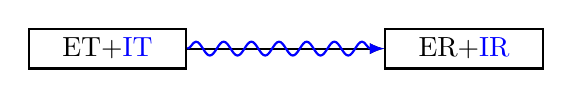
\begin{tikzpicture}[align=center,thick]
	\draw (0,0) node[draw,minimum width=2cm](t){ET+{\color{blue}IT}};
	\draw[-latex](t.east) -- ++(2.5,0) node[draw,solid,anchor=west,minimum width=2cm](r){ER+{\color{blue}IR}};
	\draw[-latex,blue,decorate,decoration=snake] (t.east) -- (r);
\end{tikzpicture}

					}
					\label{fg:swipt_colocated}
				}
				\subfloat[\gls{swipt} with separated receivers]{
					\resizebox{7cm}{!}{
						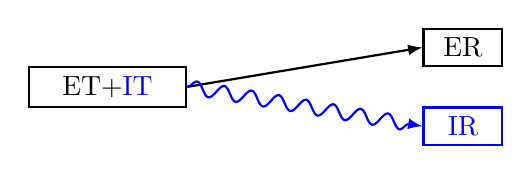
\begin{tikzpicture}[align=center,thick]
	\draw (0,0) node[draw,minimum width=2cm](t){ET+{\color{blue}IT}};
	\draw[-latex](t.east) -- (4,0.5) node[draw,solid,anchor=west,minimum width=1cm]{ER};
	\draw[-latex,blue,decorate,decoration=snake](t.east) -- (4,-0.5) node[draw,solid,anchor=west,minimum width=1cm]{IR};
\end{tikzpicture}

					}
					\label{fg:swipt_separated}
				}
				\\
				\subfloat[Monostatic backscatter]{
					\resizebox{7cm}{!}{
						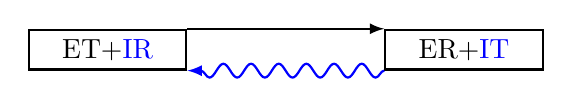
\begin{tikzpicture}[align=center,thick]
	\draw (0,0) node[draw,minimum width=2cm](t){ET+{\color{blue}IR}};
	\draw[-latex](t.north east) -- ++(2.5,0) node[draw,solid,anchor=north west,minimum width=2cm](r){ER+{\color{blue}IT}};
	\draw[-latex,blue,decorate,decoration=snake](r.south west) -- (t.south east);
\end{tikzpicture}

					}
					\label{fg:backcom_monostatic}
				}
				\subfloat[Bistatic backscatter]{
					\resizebox{7cm}{!}{
						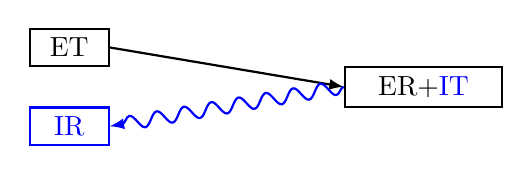
\begin{tikzpicture}[align=center,thick]
	\draw (0,0.5) node[draw,solid,anchor=west,minimum width=1cm](et){ET};
	\draw (0,-0.5) node[draw,blue,solid,anchor=west,minimum width=1cm](ir){IR};
	\draw[-latex](et.east) -- (4,0) node[draw,solid,anchor=west,minimum width=2cm](erit){ER+{\color{blue}IT}};
	\draw[-latex,blue,decorate,decoration=snake] (erit.west) -- (ir.east);
\end{tikzpicture}

					}
					\label{fg:backcom_bistatic}
				}
				\caption{
					Information and energy flows in \gls{swipt} and \gls{bc} systems. Blue and black parts denote information and power subsystems, respectively.
				}
				\label{fg:wipt_schemes}
			\end{figure}
			From a design perspective, co-located \gls{swipt} receiver is a more general model since it can exploit the received signal for either purpose or a mixture in between.
			We thus focus on this model in the following context.
		\end{subsubsection}

		\begin{subsubsection}{Receiver Architectures}
			Figure \ref{fg:swipt_receiver_architectures} illustrates four potential architectures for a co-located \gls{swipt} receiver \cite{Clerckx2022}:
			\begin{figure}[H]
				\centering
				\subfloat[Ideal receiver]{
					\resizebox{0.6\columnwidth}{!}{
						\begin{circuitikz}[transform shape,align=center]
	\draw (0,0) node[bareRXantenna](r){Rx}(r.center) to ++(0,-1) to ++(1.5,0) coordinate(j){} to ++(0,1) to ++(1,0) node[draw,anchor=west,minimum width=2.5cm](eh){Energy\\harvester};
	\draw (eh.east) to ++(1,0) node[draw,anchor=west,minimum width=2.5cm]{Power\\management};
	\draw (j) to ++(0,-1) to ++(1,0) node[draw,anchor=west,minimum width=2.5cm]{Information\\decoder};
\end{circuitikz}

					}
					\label{fg:receiver_ideal}
				}
				\\
				\subfloat[Time switching receiver]{
					\resizebox{0.6\columnwidth}{!}{
						\begin{circuitikz}[transform shape,align=center]
	\draw (0,0) node[bareRXantenna](r){Rx}(r.center)
		to[short] ++(0,-1) node[below]{Time switcher}
		to[short] node[spdt,anchor=in](s){} ++(0.5,0);

	\draw (s.out 1)
		to ++(1.25,0)
		to ++(0,0.5)
		to ++(1,0) node[draw,minimum width=2.5cm,anchor=west](eh){Energy\\harvester};
	% \draw (eh.east) to ++(1,0) node[draw,anchor=west,minimum width=2.5cm]{Power\\management};

	\draw (s.out 2)
		to ++(1.25,0)
		to ++(0,-0.5)
		to ++(1,0) node[draw,anchor=west,minimum width=2.5cm]{Information\\decoder};
\end{circuitikz}

% \begin{circuitikz}[transform shape,align=center]
% 	\draw (0,0) node[bareRXantenna](r){Rx}(r.center)
% 		to[short] ++(0,-1)
% 		to node[coupler,anchor=left up](c){Power splitter} ++(1,0);
% 	\draw (c.right up)
% 		to[short] ++(0.5,0)
% 		to ++(0,0.5)
% 		to ++(1,0) node[draw,minimum width=2.5cm,anchor=west](eh){Energy\\harvester};
% 	\draw (eh.east) to ++(1,0) node[draw,anchor=west,minimum width=2.5cm]{Power\\management};
% 	\draw (c.right down)
% 		to[short] ++(0.5,0)
% 		to ++(0,-0.5)
% 		to ++(1,0) node[draw,anchor=west,minimum width=2.5cm]{Information\\decoder};
% \end{circuitikz}

					}
					\label{fg:receiver_ts}
				}
				\\
				\subfloat[Power splitting receiver]{
					\resizebox{0.6\columnwidth}{!}{
						\begin{circuitikz}[transform shape,align=center]
	\draw (0,0) node[bareRXantenna](r){Rx}(r.center)
		to[short] ++(0,-1)
		to node[coupler,anchor=left up](c){Power splitter} ++(1,0);
	\draw (c.right up)
		to[short] ++(0.5,0)
		to ++(0,0.5)
		to ++(1,0) node[draw,minimum width=2.5cm,anchor=west](eh){Energy\\harvester};
	% \draw (eh.east) to ++(1,0) node[draw,anchor=west,minimum width=2.5cm]{Power\\management};
	\draw (c.right down)
		to[short] ++(0.5,0)
		to ++(0,-0.5)
		to ++(1,0) node[draw,anchor=west,minimum width=2.5cm]{Information\\decoder};
\end{circuitikz}

					}
					\label{fg:receiver_ps}
				}
				\\
				\subfloat[Integrated receiver]{
					\resizebox{0.6\columnwidth}{!}{
						\begin{circuitikz}[transform shape,align=center]
	\draw (0,0) node[bareRXantenna](r){Rx}(r.center) to ++(0,-1) to ++(1.5,0) node[draw,anchor=west,minimum width=2.5cm](eh){Joint harvester\\and decoder};
	\draw (eh.east) to ++(2,0) node[draw,anchor=west,minimum width=2.5cm]{Power\\management};
\end{circuitikz}

					}
					\label{fg:receiver_integrated}
				}
				\caption{
					Architectures of a co-located \gls{swipt} receiver.
				}
				\label{fg:swipt_receiver_architectures}
			\end{figure}

			\begin{itemize}
				\item \emph{Ideal receiver:} The received signal is used for both information decoding and energy harvesting. This is theoretically the most efficient design with a rectangle \gls{r-e} region but is unimplementable in practice due to hardware constraints.
				\item \emph{\gls{ts} receiver:} Each time frame is divided into individual \gls{wit} and \gls{wpt} phases, where the receiver switches between information decoder and energy harvester, respectively. The transmitted waveform and \gls{ris} response are optimized independently for each phase, and the resulting \gls{r-e} region is a triangle with two vertices corresponding to \gls{wit}-only and \gls{wpt}-only.
				\item \emph{\gls{ps} receiver:} The received signal is split into two parts with power ratio $\rho$ and $1{-}\rho$. The former is fed into the energy harvester and the latter is used for information decoding. The transmitter and \gls{ris} are jointly optimized for both purposes with the knowledge of splitting ratio, and the resulting \gls{r-e} region may be non-convex.
				\item \emph{Integrated receiver \cite{Kim2021a}:} The transmit signal is modulated in properties that can be well-preserved after rectification (e.g., pulse position) such that information can be decoded from the energy harvester output.
			\end{itemize}

			The most popular architectures in the literature are \gls{ts} and \gls{ps} due to their practicality and tractability.
			The \gls{r-e} region of the former can be inferred from that of the latter, since the \gls{wit}-only and \gls{wpt}-only vertices in \gls{ts} correspond to $\rho=1$ and $\rho=0$ in \gls{ps}, respectively.
			Integrated receiver eliminates the need of \gls{rf} chains and advanced architectures, but experiences information degradation and works better for low-throughput applications.
		\end{subsubsection}
	\end{subsection}
\end{section}

\begin{section}{\glsfmtfull{bc}}
	\begin{subsection}{Introduction}
		The scattered waves from any object inherently contain some information about the object.
		This contributed to the great success of radar in the World War II, where the ``objective'' information about the target (e.g., size, speed, and position) can be extracted from the reflected signal.
		Soon after the war in 1948, Stockman demonstrated the concept of \gls{bc} where the target is no longer a dumb wave scatterer but part of the communication system that is willing to modulates its ``subjective'' information over the reflected signal \cite{Stockman1948}.
		The communication society quickly realized its potential to separate the power-hungry \gls{rf} carrier emitter with the low-power information modulator, which is essential for miniaturizing wireless devices and increasing the network scale.
		As shown in Figs. \subref*{fg:backcom_monostatic} and \subref*{fg:backcom_bistatic} on Page \pageref{fg:wipt_schemes}, the backscatter node (a.k.a. tag) is activated by an energy signal (also functions as carrier) in the downlink and modulates over the scattered signal in the uplink. The energy transmitter (a.k.a. carrier emitter) and information receiver (a.k.a. reader) can be either co-located or separated, known respectively as monostatic and bistatic \gls{bc}.

		One of the most well-known \gls{bc} applications is \gls{rfid} which made its debut in the 1970s \cite{Landt2005}.
		\gls{rfid} readers sends a query signal and exploit the reflected signal from nodes (attached to objects) to identify and track them.
		The nodes can be powered wirelessly by the impinging wave and does not have to be in the vicinity of the reader.
		It has been standardized in ISO/IEC 18000 and EPC Gen2 \cite{Abbasi2021a} and widely used in supply chain management, access control, and asset tracking.
		On the other hand, \gls{bc} also plays an important role in emerging applications like \gls{iot}, \gls{wsn}, and \gls{m2m} communications.
		Their main difference to \gls{rfid} is that the message is no longer a static identifier but can be dynamically sensed from the environment or generated on demand.
		This enables a new paradigm of self-sustainable, intelligent, and pervasive sensing and communication, which is a key building block for our initial vision.

		Nevertheless, low throughput and limited coverage are acknowledged as two critical problems for conventional \gls{bc} systems.
		Those are inevitably inherited from the nature of wave scattering --- the radiated signal has to travel a round trip (emitter-node-reader) with double pathloss, while the scatter response is frequency-dependent and usually results in a narrow bandwidth.
		Monostatic \gls{bc} is also subject to a strong self-interference that further degrades the error performance and achievable rate.
		Finally, the nodes are idle most of the time and only respond when externally inquired.
		This is in sharp contrast to \gls{ris} where the elements are contributing for channel enhancement all the time.
		To mitigate those issues, multi-antenna techniques and special modulation schemes are two promising solutions in the literature.
		For example, a multi-antenna carrier emitter can perform energy beamforming \cite{Yang2015b}, a multi-antenna node can perform energy combining with spatial modulation \cite{Chen2020,Goudeli2020} or space-time coding \cite{Liu2021a}, and a multi-antenna reader can perform coherent \cite{He2020d,Wang2021b} or non-coherent \cite{Devineni2021} detection.
		We will discuss some popular modulation and coding techniques for \gls{bc} in the following subsection.
	\end{subsection}

	\begin{subsection}{Modulation and Coding Schemes}
		\gls{bc} and \gls{ris} share the same wave scattering model in Section \ref{sc:principles}, but the reflection coefficient $\Gamma$ in \eqref{eq:reflection_coefficient} is exploited in different manners.
		The difference is two-fold:
		\begin{itemize}
			\item \emph{Modulation requires variation:} \gls{bc} relies on dynamically changing the reflection coefficient over time to encode information. This is different from \gls{ris} where the optimal configuration (and reflection coefficient) is fixed for a given channel realization.
			\item \emph{Harvesting requires absorption:} Part of the impinging wave should be fed into the node to power its operation. This is different from \gls{ris} where a full reflection is desired to maximize its channel control capability.
		\end{itemize}
		Denote the amplitude scattering ratio of the \gls{bc} node as $\alpha$, i.e., the power absorption ratio is $(1-\alpha)^2$. Some popular modulation schemes are summarized below:
		\begin{itemize}
			\item \emph{\gls{qam} \cite{Thomas2012a}:} The reflection coefficient corresponding to the $m$-th symbol is
			\begin{equation}
				\Gamma_m = \alpha \frac{c_m}{\max_{m'} \lvert c_{m'} \rvert}
			\end{equation}
			where $c_m$ is the corresponding constellation point.
			This scheme is simple but exhibits a low detection \gls{snr} especially when the constellation size is large.
			\item \emph{\gls{fsk} \cite{Abbasi2021a}:} For 2-\gls{fsk}, the reflection coefficient is
			\begin{equation}
				\Gamma(t) =
				\begin{cases}
					\alpha, & t \in \bigl[\frac{n}{\Delta f},\frac{2n+1}{2 \Delta f}\bigr) \\
					-\alpha, & t \in \bigl[\frac{2n+1}{2 \Delta f},\frac{n+1}{\Delta f}\bigr)
				\end{cases}
				= \frac{\pi}{4} \sum_{m=1,\text{odd}}^\infty \frac{1}{m} \sin\bigl(2\pi m \Delta f t\bigr),
			\end{equation}
			where $n \in \mathbb{N}$.
			If the incident wave is a \gls{cw} at frequency $f_0$, the reflected signal is dominated by its first harmonic
			% \begin{equation}
			% 	y(t) = \sum_{m=1,\text{odd}}^\infty \frac{\pi}{4m} \cos(2 \pi f_0 t) \sin\bigl(2\pi m \Delta f t\bigr),
			% \end{equation}
			\begin{equation}
				s_1(t) = \frac{\pi}{2} \Bigl(\sin\bigl(2 \pi (f_0 {+} \Delta f) t\bigr) - \sin\bigl(2 \pi (f_0 {-} \Delta f) t\bigr)\Bigr).
			\end{equation}
			That is, periodically switching the reflection coefficient at rate $\Delta f$ results in a frequency shift $\pm \Delta f$ on the reflected signal.
			Practical implementations have been demonstrated on a variety of license-free protocols (e.g., HitchHike \cite{Zhang2016a}, Inter-Technology \cite{Iyer2016}, Passive Wi-Fi \cite{Kellogg2017}, \gls{ble}-Backscatter \cite{Ensworth2017}) where the mirror copy can be suppressed.
			\item \emph{\gls{css} \cite{Talla2017}:} A chirp is a signal whose frequency increases or decreases over time.
			\gls{css} uses wideband linear-frequency modulated chirps to encode information, which is from \gls{dsss} and \gls{fsss} with pseudo-random sequences and \gls{fsk} with discrete frequencies.
			In particular, $N+1$ reflection coefficients of the same envelope are sequentially selected at a regular rate $\Delta f$, given by
			\begin{equation}
				\Gamma_n = \alpha \exp(\jmath \phi_n), \quad n \in \{0, 1, \ldots, N\},
			\end{equation}
			where $\phi_n = \frac{2 \pi}{\Delta f}(A n^2 + B n)$ and $A$, $B$ are constants.
			As the core modulation scheme in \gls{lora}, it is more robust to noise and interference (with a reception sensitivity of -149 dBm), harder to be detected by eavesdroppers, and can be used for ranging and localization \cite{Abbasi2021a}.

			Common \gls{bc} channel coding schemes include unipolar \gls{rz} and \gls{nrz}, Manchester, differential, pulse-pause and FM0.
			They are not the focus of the thesis and the readers are referred to \cite[Chapter 2.3]{Hoang2020} for details.
		\end{itemize}
	\end{subsection}

	\begin{subsection}{Applications}
		\begin{subsubsection}{\glsfmtfull{mbc}}

		\end{subsubsection}

		\begin{subsubsection}{\glsfmtfull{bbc}}

		\end{subsubsection}

		\begin{subsubsection}{\glsfmtfull{ambc}}

		\end{subsubsection}

		\begin{subsubsection}{\glsfmtfull{sr}}

		\end{subsubsection}
	\end{subsection}
\end{section}

% \begin{section}{\glsfmtfull{im}}

% \end{section}

% \begin{section}{\glsfmtfull{mimo}}
% 	\begin{subsection}{\glsfmtfull{pc}: Channel Shaping}

% 	\end{subsection}

% 	\begin{subsection}{\glsfmtfull{ic}: Interference Alignment}

% 	\end{subsection}
% \end{section}
